\chapter{Background}

\section{Magnolia}

Magnolia is an experimental research language being developed \gls{bldl} at the
University of Bergen. Magnolia is designed to support a high level of abstraction
and ease of reasoning. This is achieved by \textit{concepts}, \textit{axioms} and
\textit{implementations}.
\todo{expand}

\subsection{Group}

\todo{Tie these two sections together}

Something, something\dots string concatenation is actually a semigroup. Which is
helpful because reasons

\todo{Tie these two sections together}

Sets with specific operations acting on those elements, known as algebraic
structures, showcase the usage of concepts. Magma consists of a set with just a
singular binary operation, that must be closed by definition. A semigroup is an
extension of magma, with the added property that the binary operation is
associative. A monoid is an extension of a semigroup, with the added property
wherein an element in the set, \textit{C}, sometimes called a \textit{unit}, or
the \textit{identity}. This \textit{identity} ensures the following equation
holds, where the binary operation is $ \oplus $, and $ a, C $ are elements of the set.

\begin{equation}
  a \oplus C = a
\end{equation}

This, again, can be extended with an additional property, namely,
\textit{inverse element}.

\begin{equation}
  \forall a, \exists b, \in M \implies a \oplus b = C
\end{equation}

Assuming associativity.

\subsubsection{Java Group}

This structure not could be implemented in something like Java, an
Object-Oriented Language, as shown in listings \ref{lst:jmagma},
\ref{lst:jsemigroup}, \ref{lst:jmonoid}, and \ref{lst:jgroup}. Note the empty
interfaces; there is nothing that enforces the different laws on the properties.
This can only be done by unit testing, which is not enforced on a consumer of
the \gls{api}.

\begin{center}
  \lstinputlisting
    [ language=Java
    , caption={Magma concept in Java}
    , label=lst:jmagma]{./code/magma.java}
\end{center}

\begin{center}
  \lstinputlisting
    [ language=Java
    , caption={Semigroup concept in Java, can only be upheld using unit tests}
    , label=lst:jsemigroup]{./code/semigroup.java}
\end{center}

\begin{center}
  \lstinputlisting
    [ language=Java
    , caption={Monoid concept in Java, can only be upheld using unit tests}
    , label=lst:jmonoid]{./code/monoid.java}
\end{center}

\begin{center}
  \lstinputlisting
    [ language=Java
    , caption={Group concept in Java, can only be upheld using unit tests}
    , label=lst:jgroup]{./code/group.java}
\end{center}


\subsubsection{Haskell Group}

\todo{Add examples}

This can also not be implemented in Haskell

\subsubsection{Magnolia Group}

In Magnolia, however, this can be enforced on the \textit{interface}-level. The
example code shown in listing \ref{lst:magma}, showcases a concept
representation a binary operation, which has one function, \textit{magma}, which
takes in two values of type \textit{T}, and returns \textit{T}. Note that the
actual implementation of this function is missing. This is because a concept
encodes the properties of a users code. The actual implementation of the
\textit{magma} function needs to uphold the properties of the concept that is
being implemented. In this case, it is just that the input and output
of the function are of the same types.

\begin{center}
  \lstinputlisting
    [ language=Magnolia
    , caption={Magma concept in Magnolia}
    , label=lst:magma]{./code/magma.mg}
\end{center}

In the example code shown in listing \ref{lst:semigroup}, the \textit{magma}
concept has been expanded upon, still following the same rules as before, but
with the added property of associativity.

\begin{center}
  \lstinputlisting
    [ language=Magnolia
    , caption={Semigroup concept in Magnolia}
    , label=lst:semigroup]{./code/semigroup.mg}
\end{center}

\begin{center}
  \lstinputlisting
    [ language=Magnolia
    , caption={Monoid concept in Magnolia}
    , label=lst:monoid]{./code/monoid.mg}
\end{center}

\begin{center}
  \lstinputlisting
    [ language=Magnolia
    , caption={Group concept in Magnolia}
    , label=lst:group]{./code/group.mg}
\end{center}

So Magnolia facilitates \textit{reuse}.
\todo{Make the red-thread easier to follow}

\section{Reusable Software}

One of the most important features in any programming language, is the notion
of \textit{reusability}. From the invention of the GO-TO-statement,
to functions, and external libraries, being able to reuse existing software is
an important tool for a developer. It avoids \textit{re-inventing the wheel}, as
common functionality can be externalized and reused in several different places.

\subsection{Reuse in Magnolia}

Reusability is also an important feature in Magnolia, but this reusability is in
the entire language. In libraries in other languages, functions are reused, in
an attempt to avoid common logical mistakes, but these mistakes could still be
there, hiding in plain view. In Magnolia, one can re-use the \textit{logic} of a
function.
\todo{Expand}

\subsection{Software Lifetimes}

Software in general, lasts around 30 years (source). This is quite a long time,
but, this statistic is about more \textit{rigid} applications, which have an
unchanging scope. In more \textit{chaotic} fields, this number is reduced, as
paradigm shifts within certain fields, which results in the need for drastic
changes in the existing applications, where the needed work to change the code,
can be more than to create a new application.

\subsection{Software Longevity}

Most examples of \textit{popular} software, are open source, like \gls{vim}.
\gls{vim} is a text editor which has been in use since 1991. There are several
factors behind this success, but the ones being highlighted here, are due to its
extensibility and due to it being open-sourced. Being open sourced, allows for a
rotating cast of maintainers, ensuring the core application has the features its
users wants. The users of \gls{vim} can be split into two categories,
\textit{standard users}, and \textit{module developers}. \gls{vim} has an
extensive module ecosystem, which can extend \gls{vim}s functionality from a
text editor, to a fully fledged \gls{ide}.

\section{Integrated Development Environment}

An \gls{ide}, aids a developer, as all the needed tools for development are
integrated into one application. There are two different kinds of \gls{ide}s,
generic and specialized. \todo{Source}

A specialized \gls{ide} is one targeted towards a specific language, like
Eclipse, (reference?), or IntelliJ (reference?), which target Java/JVM. It
contains specialized features like the following:

\paragraph{Syntax Highlighting} Highlighting important keywords, identifiers
and more, makes the language easier to read for the developer, allowing them to
spot easy to miss errors, like misspelling of keywords.

\paragraph{Code Autocompletion} Suggesting keywords, method names or even entire
code snippets, is a powerful tool an \gls{ide} can have. This is possible to
achieve, in some form, without being specialized, by for example, suggesting
text that already exist in the document, but is most useful if it is
specialized, and can suggest built-in methods. This allows a developer to not
having to remember exactly how methods are named, is the method to split a
string by some delimiter, \textit{split\_by} or \textit{split\_on}? As long as
the developer writes \textit{split}, the correct method name will be suggested.

\paragraph{Go-To-Definitions} Being able to quickly navigate to methods and read
their implementation is a useful tool for a developer, as less time has to be
spent navigating the project structure, to figure out where some method was
implemented, and more time can be spent actually developing.

A lot of these features are possible due to \textit{Language Server Protocols},
which allow for a standardized way for compilers to give code-support to
\gls{ide}'s.

A generic \gls{ide} contains the features that are common among development in
any programming language, like:

\paragraph{File Explorer} Most project nowadays is larger than one file, so
being able to visualize the project in a tree-like-structure, and navigate that,
is useful. This feature usually comes with the ability to manipulate the project
structure, by adding files, folders, moving files around, and deleting them.

But creating any \gls{ide} would still limit the lifetime of the application.
The best example of a long living active \gls{ide}, or, at least editor, is Vim
(source?). Vim is not a feature full editor, but it is simple, lightweight, and
works on any operating system. But most people use it, for how easy it is to
extend; Its lifetime has been greatly extended by the ease of modularization.
Any popular module for Vim is open-source, and therefore, if any module had an
active community around it, if the \textit{lead} developer of the module stopped
developing it, that community can continue to develop the module, either by
getting maintenance access to the repository, or by forking it. Ensuring the
lifetime of the module is extended.

\subsection{Module Architecture}

\todo{Talk about modules in IDEs}

\subsection{Module Ecosystem}

\todo{Expand}
More modules == better, right?

\subsection{Granularity}

When designing modules, the \textit{granularity} of the combined modules has to
be considered. As an example, if one where to extend the zero-core application
with the needed functionality for it to be considered an \gls{ide}, this could be
achieved by creating a singular module which does all the work. However, this
is not a modular approach, as if one wants to change some specific feature in
the \gls{ide}-module, one would have to re-create the whole module with that
specific feature implemented. Instead, if this functionality was granular,
that is to say, split into several modules, that together enable the needed
features, then it would be \textit{simpler} to modify the needed modules to
achieve the wanted feature.


\subsection{Module Family}

\begin{figure}
  \centering
  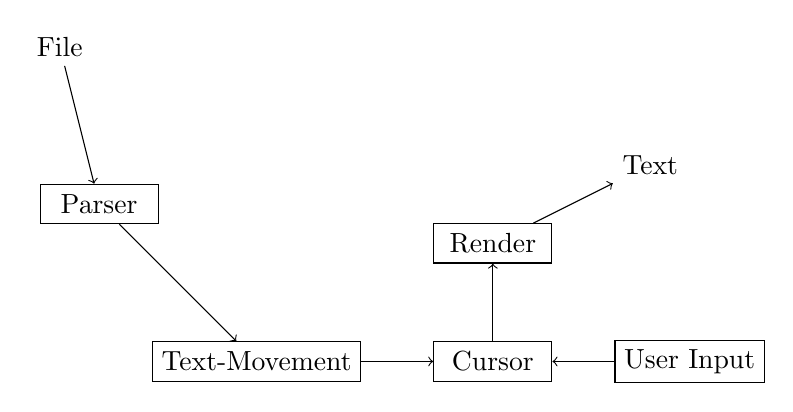
\begin{tikzpicture}
  % Nodes
  \node (file) [] at (-6, 3) {File};
  \node (parser) [rectangle, draw, minimum height=0.5cm, minimum width=1.5cm] at (-5.5, 1) {Parser};
  \node (text-movement) [rectangle, draw, minimum height=0.5cm, minimum width=1.5cm] at (-3.5, -1) {Text-Movement};
  \node (cursor) [rectangle, draw, minimum height=0.5cm, minimum width=1.5cm] at (-0.5, -1) {Cursor};
  \node (user-input) [rectangle, draw, minimum height=0.5cm, minimum width=1.5cm] at (2, -1) {User Input};
  \node (render) [rectangle, draw, minimum height=0.5cm, minimum width=1.5cm] at (-0.5, 0.5) {Render};
  \node (text) at (1.5, 1.5) {Text};
  % Arrow
  \draw[->] (file) -- (parser) node[midway, above] {};
  \draw[->] (parser) -- (text-movement) node[midway, above] {};
  \draw[<-] (cursor) -- (text-movement) node[midway, above] {};
  \draw[<-] (cursor) -- (user-input) node[midway, above] {};
  \draw[->] (cursor) -- (render) node[midway, above] {};
  \draw[->] (render) -- (text) node[midway, above] {};
\end{tikzpicture}

  \caption{Text Editor Module Family}
  \label{fig:textEditorSimple}
\end{figure}

In figure \ref{fig:textEditorSimple}, an input file is parsed to some structure
which is used to translate user actions, into cursor movements. The cursor being
the place in the file where text is written to by the user.

This is a feature that naturally shows up in a \textit{true} modular system. If
several modules together enable some feature, then those modules can be treated
as a singular module by an external module developer, depending on what they
want to extend.

\subsection{Language Workbench}
\todo{Expand}
I don't know what this is.

\subsection{Language Server}

The most important features in a modern \gls{ide} are possible due to the
\gls{lsp}. \gls{lsp} is a protocol for a language server and editor,
(the client), with which they communicate, allowing for features like code
completion, syntax highlighting, marking of warnings and errors, as well as
refactoring routines. This client-server architecture, in \gls{ide}s are a
more recent development (2020s), as previously, support for the features
mentioned, were only possible due to specific modules being written for
specific \gls{ide}s. \gls{lsp} being the norm, is a sign of modularity being
preferred, as now a single \gls{lsp} can be created, and used across several
different applications, like IntelliJ, VS Code and Vim. While useful for
\textit{standard} language, this is the limiting factor when it comes to
supporting experimental languages, as not only does a new set of protocols need
to be appended to a language server, the editor itself needs to be changed to
actually use these protocols. This creates a lot of work, for both the \gls{ide}
developer and for the compiler developer. Here is where a modular approach can
help both. If some new functionality or feature is added to the experimental
language, this off course means the compiler/interpreter has to be expanded
and/or modified, but for the \gls{ide}, a module could be added/modified to
utilize this change, instead of having to change the entire application.

\section{Existing Magnolia IDE}

The current \gls{ide} for Magnolia, is a many-years-old version of Eclipse,
using modules and functionality from the core Eclipse application, that has
since been outdated. The \gls{ide}s lifetime was limited by a dependency on
external modules and features that where not maintained by the
\gls{ide}-developers. This meant that for future development of Magnolia, an
outdated \gls{ide} was needed, with outdated tooling. Furthermore, the Magnolia
compiler was implemented as an Eclipse module, which means that development is
limited to Eclipse, and only Eclipse, as a developer cannot compile Magnolia
code without it.

Modularization will help to mitigate some of the issues with the current
Magnolia \gls{ide}. Instead of maintaining an entire application, the needed and
wanted features of the application can be maintained instead.

Experimental languages might have features which are not possible to be fully
used in current \gls{ide}s. This is also the case for the current Magnolia
\gls{ide}. The compiler for Magnolia, syntax highlighting, error reporting, and
hover-functionality are functionality made in the Eclipse \gls{ide}, by using
its plug-in architecture. Some of the functionality and plug-ins this
implementation used, have been deprecated in later version of Eclipse. This
means the Magnolia \gls{ide} is locked to an old version of Eclipse, which, as
time passes, increases the complexity of installation, as the surrounding
tooling and libraries needed by this version of Eclipse also becomes deprecated.
Currently, in INF220, at the university, two weeks are set aside for students to
be able to install it.

\todo{Reference Anya's paper}
